\newpage
\subsection*{Part 1 - Building a Database for Concordia Foundation}

\begin{enumerate}[label={(\alph*)}]
    \item In the \textit{Assigned} relationship, not all organizations are necessarily assigned a project, and organizations can be assigned multiple projects, hence the line from \textit{Organizations} to \textit{Assigned} is thin and do not have an arrow. However, for the line between \textit{Assigned} and \textit{Projects}, we are told that each project is assigned \textbf{to one and only one} organization. That means that it is a one-to-many total relationship. The line from \textit{Projects} to \textit{Assigned} is thick (total) ans has an arrow (one-to-many). Note that we are assuming that a project has to be assigned to a Organization, that why we use a total relationship. Here is the corrected ER diagram representing the \textit{Assigned}. 
    
    \begin{center}
        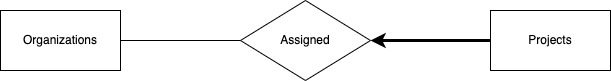
\includegraphics[width=0.9\textwidth]{img/1a.jpg}
    \end{center}
    
    \item Bellow is the full ER diagram for the C.F. database.
    \begin{center}
        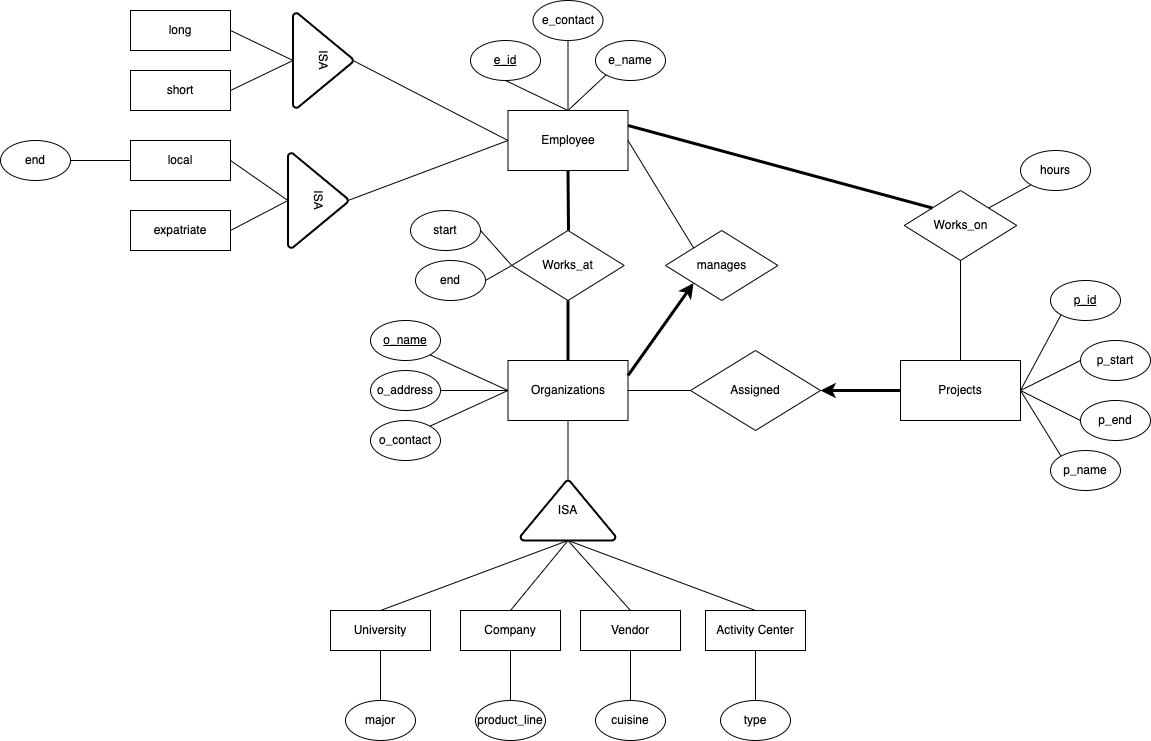
\includegraphics[width=1\textwidth]{img/1b.png}
    \end{center}
    We are assuming that all organizations have at least one employee. 
    
    \item Since the organizations are classified as either a university, a company, a vendor, or a activity center, we can say that these 'categories' cover all the instances of the Organizations entity set. An organization cannot be classified as two different type. The four possible types of organization are disjoint subsets of the Organization entity set. Hence, the Organizations ISA hierarchy has covering constraints. 
    
    \item First, we know that the \textbf{long} and \textit{short} subsets cover \textit{Employees}. We also know that The \textbf{local} and \textit{expatriate} subsets cover \textit{Employees}. However, \textbf{long}, \textbf{short}, \textbf{local}, and \textbf{expatriate} subsets overlap employee since \textbf{long} and \textbf{short} are not disjoint from \textbf{local} and \textbf{expatriate}. For example, a long term employee can be expatriate while another long term employee is local. 
    
    \item \begin{verbatim}
        CREATE TABLE Organizations(
            o_name: CHAR(20) NOT NULL,
            o_address: CHAR(20),
            o_contact: CHAR(20),
            PRIMARY KEY (o_name),
            UNIQUE (o_name)
            );
        
        CREATE TABLE Employees(
            e_id: CHAR(20) NOT NULL,
            e_contact: CHAR(20),
            e_name: CHAR(20),
            PRIMARY KEY (e_id),
            UNIQUE (e_id)
            );
            
        CREATE TABLE Projects(
            p_id: CHAR(20) NOT NULL,
            p_start: DATE,
            p_end: DATE
            p_name: CHAR(20),
            PRIMARY KEY (p_id),
            UNIQUE (p_id)
            );
        
        CREATE TABLE University(
            o_name: CHAR(20) NOT NULL,
            major: CHAR(20)
            PRIMARY KEY (o_name),
            FOREIGN KEY (o_name) REFERENCES Organizations 
            );
        
        CREATE TABLE Company(
            o_name: CHAR(20) NOT NULL,
            product_line: CHAR(20)
            PRIMARY KEY (o_name),
            FOREIGN KEY (o_name) REFERENCES Organizations 
            );
            
        CREATE TABLE Vendor(
            o_name: CHAR(20) NOT NULL,
            cuisine: CHAR(20)
            PRIMARY KEY (o_name),
            FOREIGN KEY (o_name) REFERENCES Organizations 
            );
            
        CREATE TABLE Activity Center(
            o_name: CHAR(20) NOT NULL,
            type: CHAR(20)
            PRIMARY KEY (o_name),
            FOREIGN KEY (o_name) REFERENCES Organizations 
            );
        
        CREATE TABLE Works_at (
            o_name: CHAR(20) NOT NULL,
            e_id: CHAR(20) NOT NULL,
            end: DATE,
            start: DATE,
            PRIMARY KEY (o_name, e_id),
            FOREIGN KEY (o_name) REFERENCES Organizations,
            FOREIGN KEY (e_id) REFERENCES Employees
            );
        
        CREATE TABLE Works_on (
            p_id: CHAR(20) NOT NULL,
            e_id: CHAR(20) NOT NULL,
            hours: TIME,
            PRIMARY KEY (p_id, e_id),
            FOREIGN KEY (p_id) REFERENCES Projects,
            FOREIGN KEY (e_id) REFERENCES Employees
            );
            
        CREATE TABLE Assigned (
            o_name: CHAR(20) NOT NULL,
            p_id: CHAR(20) NOT NULL,
            PRIMARY KEY (p_id, o_name),
            FOREIGN KEY (p_id) REFERENCES Projects,
            FOREIGN KEY (o_name) REFERENCES Organizations
            );
            
        CREATE TABLE Manages (
            o_name: CHAR(20) NOT NULL,
            e_id: CHAR(20) NOT NULL,
            PRIMARY KEY (e_id, o_name),
            FOREIGN KEY (e_id) REFERENCES Employees,
            FOREIGN KEY (o_name) REFERENCES Organizations
            );
        
        CREATE TABLE long (
            e_id: CHAR(20) NOT NULL,
            PRIMARY KEY (e_id),
            FOREIGN KEY (e_id) REFERENCES Employees
            );
            
        CREATE TABLE short (
            e_id: CHAR(20) NOT NULL,
            PRIMARY KEY (e_id),
            FOREIGN KEY (e_id) REFERENCES Employees
            );
            
        CREATE TABLE local (
            e_id: CHAR(20) NOT NULL,
            end: DATE,
            PRIMARY KEY (e_id),
            FOREIGN KEY (e_id) REFERENCES Employees
            );
            
        CREATE TABLE expatriate (
            e_id: CHAR(20) NOT NULL,
            PRIMARY KEY (e_id),
            FOREIGN KEY (e_id) REFERENCES Employees
            );
    \end{verbatim}
    
    
\end{enumerate}